The internal constitution of the Earth has been investigated 
systematically from the nineteenth century on.
With the advent of seismological instrumentation for
the registration of tele-seismic events,
by the end of that century, the main tool for
obtaining direct information about distribution of the material 
properties controling seismic wave propagation became available.
Before this, mainly global properties could be determined from
gravity and magnetic field observations, astronomical data and 
indications about the heatflow from the Earth's interior.
As a result of the early seismological investigations the
main internal structure of the Earth was revealed within the 
first few decades of the twentieth century with the discovery of the
earth's core in 1906 by Oldham and Gutenberg (1912) and the solid 
inner core in 1936 by Lehmann. 

From the radial distribution of the seismic velocity profile, 
obtained by processing the tables of 
traveltime versus epicentral distance, Williamson and Adams (1923) \cite{wiad23}
made a first estimate of the density profile for a compressible
homogeneous mantle model,
consistent with the total mass of the Earth
and obtained at the same time strong indication 
for a high density core, compositionally distinct from the mantle.
They concluded that "It is therefore impossible to explain the high density of the Earth 
on the basis of compression alone. The dense interior cannot consist of ordinary rocks 
compressed to a small volume; we must therefore fall back on the only reasonable alternative, 
namely, the presence of a heavier material, presumably some metal, which, 
to judge from its abundance in the Earth's crust, in meteorites and in the Sun, is probably iron."
 
Bullen\footnote{Keith Edward Bullen (29 June 1906 – 23 September 1976) was a 
New Zealand-born mathematician and geophysicist. He is noted for his seismological interpretation of 
the deep structure of the Earth's mantle and core.} (1975) \cite{bull75} 
further refined the analysis and showed the assumption 
of a homogeneous mantle to be inconsistent with the known moment of 
inertia of the Earth.
In the 1940s and 1950s he introduced a global divison of the
Earth in concentric shells, labelled A through G, ranging from the
Earth's crust (A), bounded by the moho discontinuity, 
to the inner core (G).
Region C between, roughly 400\si{\kilo\metre} and 900\si{\kilo\metre}, 
characterized by rapid 
increase of the seismic velocities, was identified by Bullen as
a transition region between the upper mantle region B and a
homogeneous lower mantle, region D.
The deduced inhomogeneity of the mantle was projected by Bullen in this
C region. 
E through G were used to label subdivisions of the core.
Region E indicated the liquid, adiabatic outer core,
F a transition region between inner and outer core and G the solid
inner core.
Birch (1952) \cite{birc52} published improved equations of state,
based on finite-strain theory,
thereby giving a more firm physical basis to interpretation of 
available data in terms of a compressible medium.
  
In the second half of the twentieth century the resolution and 
accuracy of the models were further improved using 
continuously improved seismological observations and a growing 
data set.
It also became possible to obtain independent information about
the radial density distribution from spectral analysis of 
radial eigen-vibrations of the Earth after very large earthquakes.
This development resulted in the publication of the 
Preliminary Reference Earth Model (PREM) by Dziewonski and Anderson (1981) \cite{dzan81}
which still serves as a global reference.

The improved seismologial models indicated
that the continuous rapid velocity increase in the transition zone (C) 
was actually a succession of several abrupt changes,
confirming radial inhomogeneity in mineral phase and possibly in 
chemical composition of the mantle.
 
From geological and cosmochemical arguments a probable composition of 
the Earth had been derived consisting of a mantle with major element
composition dominated by magnesium-iron silicates and an iron-nickle
core with a small amount of lighter elements mixed in,
most likely including mainly sulphur. 
In the 1960s this resulted in the definition of a so-called
pyrolitic composition of the mantle by Ringwood
which could explain the main
mantle petrological observations regarding the complementary
nature of basalts and ultra mafic mantle rocks found in ophiolites, 
kimberlites and mantle perioditite bodies
(Ringwood, 1975 \cite{ring75}). 

In experimental high-pressure and temperature work on the 
candidate mantle materials a series of phase transitions were found
at pressure and temperature values relevant for the Earth's mantle
which could be related to the seismic discontinuities 
revealed by the seismological data.
From these the most prominent at approximately 410 and 660\si{\kilo\metre} depth 
were identified as the phase transition of the olivine component 
$\mathrm{(Mg,Fe)_2 SiO_4}$
of the pyrolitic mantle
to a denser wadsleyite crystal structure and,
at 660\si{\kilo\metre}, a transition (dissociation) from a $\gamma$-spinel 
(known as ringwoodite) structure to a two-phase assemblage, 
post-spinel, i.e.
magnesium-iron perovskite, 
$\mathrm{(Mg,Fe)SiO_3}$ and w\"{u}stite $\mathrm{(Mg,Fe)O}$. 

It was also found that the 660 km boundary corresponds to an
endothermic phase transition which would have implications for 
large scale circulation in the mantle, leading to long-standing 
speculations about the degree of layering in mantle convection
(Christensen \& Yuen (1985) \cite{chyu85},
Albarede \& van der Hilst (2002) \cite{alva02}), \url{http://www.mantleplumes.org}.

A more recent development in this area is the discovery of a new phase
transition of magnesium-perovskite to a denser form for pressure
temperature conditions, approximately 125 GPa 2500 K, relevant for the D"
layer close to the core-mantle boundary
(Lay et al., 2005, van der Hilst et al., 2007).

\begin{center}
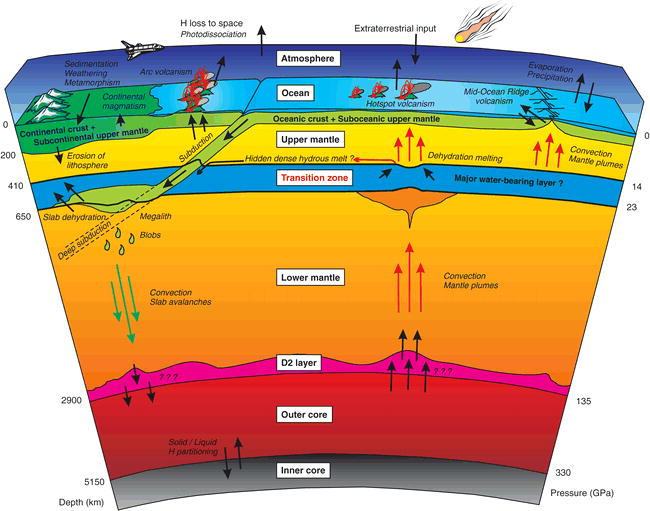
\includegraphics[width=12cm]{images/gravity/effect}\\
{\captionfont Effect of water on the phase relations in Earth's mantle and deep water cycle,\\
Litasov \& Ohtani (2007) \cite{lioh07}} 
\end{center}


~\\
In the following sections the density distribution in the
Earth's interior is treated in relation to the gravity field
and internal pressure distribution of a self-gravitating compressible
planet model and the link is shown with results from theoretical
mineral physics and high pressure-temperature experimental data for
mantle materials.
